\section{Checks}
Here we compare the results we obtain with others. 
\subsection{Gorham shower}
Gorham shower, or the reference  shower is a vertical, \unit[$\rm 3.36
  \  10^{17}$]{eV}  shower,   observed  at  \unit[10]{km}.   The  flux
originally  calculated in~\cite{gorham} is  \unit[$\rm F_{ref}  = 2.77
  \ 10^{-24}$]{$\rm W.m^{-2}.Hz^{-1}$}.   \\ We simulate the reference
shower and record the flux at several distances. The results are given
in figure~\ref{refshower}.  We have set the units the same way than in
in~\cite{imen2016}.
\begin{figure}[ht!]
  \centering
  \hspace*{-3ex}
  \subfigure{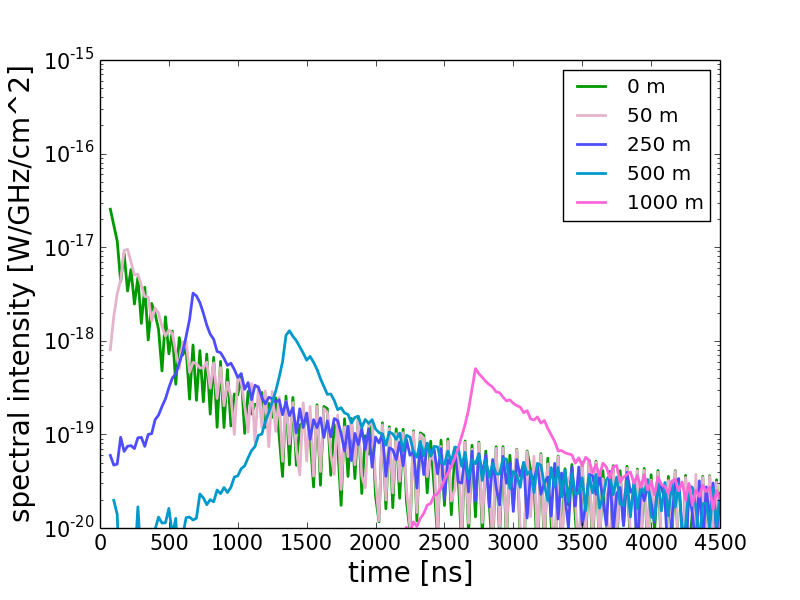
\includegraphics[width=0.49\linewidth]{myrefshower.png}}
  \subfigure{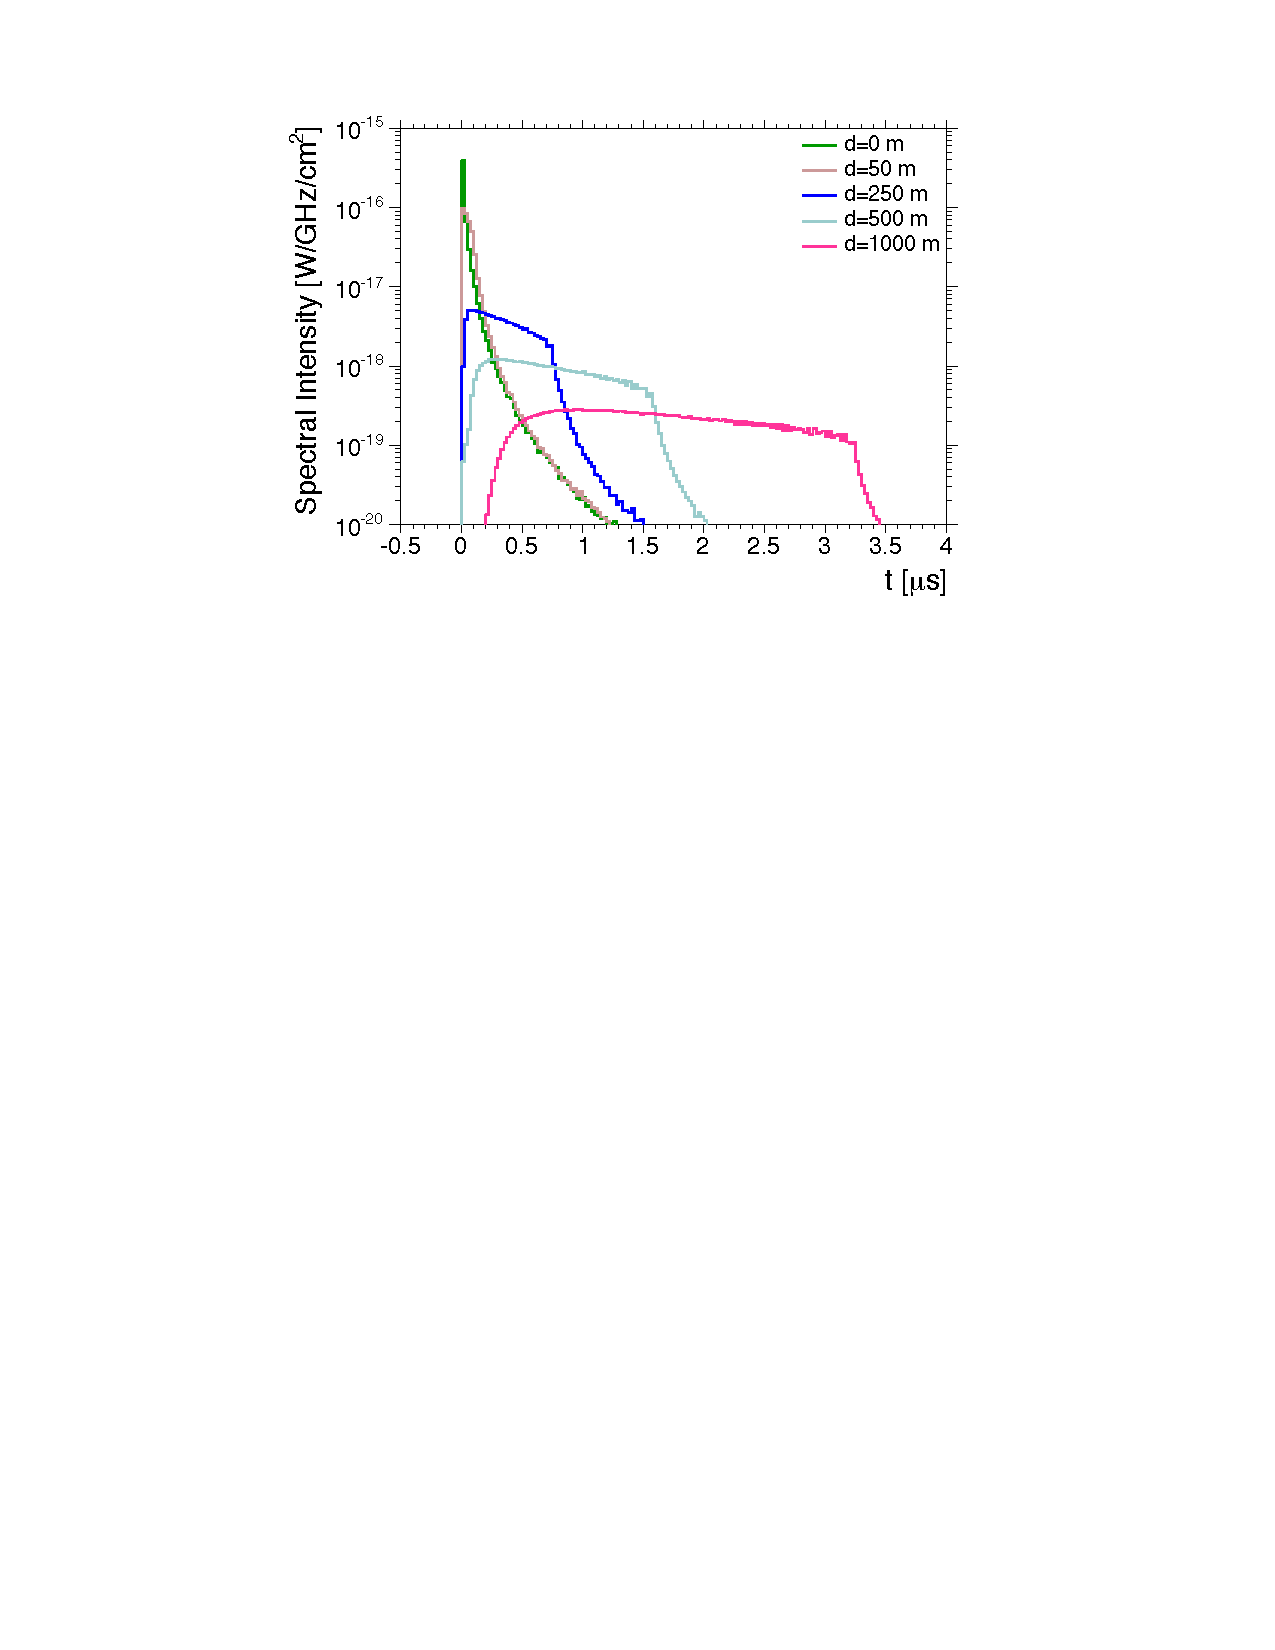
\includegraphics[width=0.49\linewidth]{paperrefshower.pdf}}
  \caption{three example of simulated trace with on top of each figure
    the signal in ADC counts, and on the bottom the signal in sigma}
  \label{fig:traceex}
\end{figure}
